\section{Overview}

This chapter describes current state of things in MIR and other fields related to the project. First, I go through the MIREX framework, giving brief overview of its structure and issues. I also describe some notable datasets that are actively used in the MIR field, how they were built, and what problems they have. In addition to that, I provide some information about how datasets in MIR and other fields are generally created and evaluated. In the end conclusions are made and ideas for work that can be done in this project are outlined.

\section{MIREX}

\subsection{Overview}

Music Information Retrieval Evaluation eXchange (MIREX) is the framework for the formal evaluation of MIR systems and algorithms \cite{downie2008mirex}. It is coordinated and managed by the International Music Information Retrieval Systems Evaluation Laboratory\footnote{\url{http://music-ir.org/}} (IMIRSEL) at the University of Illinois at Urbana-Champaign\footnote{\url{http://illinois.edu/}}.

MIREX is a direct descendant of ``Audio Description Contest'', which was convened by the Music Technology Group (MTG) at Universitat Pompeu Fabra in 2004 \cite{ismir2004description}. Both were inspired by Text Retrieval Conference (TREC) framework \cite{voorhees2005}.

All these frameworks try to standardise tasks that are performed on test collections of significant size and evaluation methods used to assess the quality of results. In case of MIREX, set of tasks and evaluation methods is largely determined by the community discussion. After community and organizers settle on what tasks they want to have as a part of next MIREX challenge, evaluations are run in July and August. Results are presented at the International Society of Music Information Retrieval (ISMIR) conference. The whole process takes about a year.

\subsection{Evaluation process}

One significant difference between TREC and MIREX is that datasets for each task are not freely distributed to the participants. All the data is stored in one central location at IMIRSEL. There are several reasons for this. Two most important are:
\begin{enumerate}
    \item Avoiding the possibility of participants to tune their algorithms specifically for the dataset.
    \item Current state of intellectual property copyright enforcement.
\end{enumerate}
Second reason generally affects MIR research in a negative way, making it harder to collect music datasets and experiment with them.

The way MIREX challenge works then is by gathering algorithms from all the participants and running them on organizer's infrastructure. All this introduces several significant challenges:
\begin{enumerate}
    \item A lot of time is spent finding, obtaining, and managing data for evaluation.
    \item Creating ground-truth data of a good quality takes a lot of resources.
    \item There is a high chance of having errors in annotations of ground-truth data and test collections.
    \item Algorithm-to-data model causes issues with capacity. Apart from terabytes of raw audio data, some algorithms that are run on this data require significant amount of intermediary storage.
    \item It takes a lot of time to manage submitted algorithms.
\end{enumerate}

According to the MIREX overview paper \cite{downie2008mirex}, there are several key issues that need to be addressed:
\begin{enumerate}
    \item Resource accessibility (music collections, ground-truth sets, pre-built models, etc.).
    \item Discovery tools for resources.
    \item Sharing and re-use of resources.
    \item Resource customization and integration.
\end{enumerate}

\section{Datasets}
\label{sec:soa:datasets}

\subsection{Overview}

\begin{table}[h]
    \footnotesize
    \centering
    \begin{tabular}{l|l|l}
        Name & Type & Size \\
        \hline
        GTZAN & Genre & 1,000 items (10 labels) \\
        ISMIR2004 Tempo Classification Dataset & Ballroom music styles & 698 items (8 labels) \\
        Music Audio Benchmark Dataset (Dortmund) & Genre & 1,886 items (9 labels) \\
        MIREX Audio Mood Classification Dataset & Mood & 1,250 items (5 clusters) \\
        MagnaTagATune & Similarity & 25,863 items (30s) \\
        The Million Song Dataset & Metadata and audio features & 1,000,000 items \\
    \end{tabular}
    \caption{Notable datasets used in MIR}
    \label{tab:mirdatasets}
\end{table}

\subsubsection{GTZAN}

GTZAN \cite{tzanetakis2002} is a dataset for music genre recognition (MGR) research, created in 2002. It has several problems: repetitions, mislabelings, and distortions \cite{sturm2013gtzan}. It is created by one person, which produces bias. It's not very diverse: many tracks are by the same artist and/or from the same album. Other major fault that is often pointed out is its size. It contains 1,000 excerpts, which is much less compared to some personal music collections (thousands of recordings) or commercial datasets and library archives (millions of recordings). It is also significantly outdated. Despite all these problems it is still one of the most actively used datasets in MGR.

\subsubsection{ISMIR2004 Tempo Classification Dataset}

ISMIR2004 Tempo Classification Dataset \cite{ballroom} was a part of audio description contest at ISMIR 2004\footnote{\url{http://ismir2004.ismir.net/ISMIR_Contest.html}}. It consists of 698 excerpts of a ballroom dance music and was meant to be used for tempo (BPM) induction. The music itself was collected from the website \href{http://www.ballroomdancers.com}{BallroomDancers.com}.

\subsubsection{Music Audio Benchmark Dataset}

Music Audio Benchmark Dataset\footnote{\url{http://www-ai.cs.uni-dortmund.de/audio.html}} \cite{dortmund} (also known as ``Dortmund'' dataset) is a dataset for genre classification. It consists of 10 seconds samples (drawn from a random position) of 1,886 songs which were obtained from the Garageband.com website. It contains 9 genre labels and additional metadata. Metadata includes information like total length, name of the band or artist, information about genre, user comments, and lyrics (partially). In addition, it provides 24 cluster models created manually by a group of users using arbitrary personal viewpoints.

This dataset also contains additional classification schemes created by users. They vary in size and cover different subsets of songs. Users classified songs according to aspects like genre, quality, preference, time of day, instruments, singer, etc.

\subsubsection{MIREX Audio Mood Classification Dataset}

MIREX Audio Mood Classification Dataset \cite{hu2007exploring,hu2008} was created to serve the need of automated classification of mood in music recordings. It was derived from metadata from AllMusicGuide.com website which, at the time, provided reviews and metadata for artists, albums, and songs. 

It consists of 5 mood clusters, each containing some specific ``mood spaces''. For example, one of the clusters contains the following ``mood spaces'': visceral, volatile, fiery, aggressive, tense/anxious, intense.

Tracks for this dataset were selected from the Associated Production Music (APM)\footnote{\url{http://www.apmmusic.com/}} collection, which is available to the MIR community under a contract of academic use between APM and IMIRSEL. From original collection of 206,851 tracks 1250 were selected (250 in each cluster). Each track there is annotated with various metadata fields like category (mood and other descriptors), instrumentation, tempo, style, and others. Selection was done by applying a number of filtering steps:
\begin{enumerate}
    \item Removal of tracks without genre information to be able to explicitly select tracks from different genres.
    \item Matching mood-related descriptors to specific clusters.
    \item Removal of tracks shorter than 50 seconds to avoid inclusion of non-music content.
    \item Removal of tracks from the same CDs to improve variety.
\end{enumerate}

In addition to original dataset, ground-truth set of 600 tracks was created. Labeling was done by people using a web service designed for MIREX evaluations - Evalutron 6000 \cite{gruzd2007evalutron}. People were instructed to ignore lyrics, since music processing technology was not sufficiently developed to transcribe them and use for classification. They were also trained on a set of examples for each mood cluster. If none of the clusters were appropriate, people could select category ``Other''. In the ground-truth set only tracks with at least two agreed labelings were used.

\subsubsection{MagnaTagATune}

MagnaTagATune\footnote{\url{http://mirg.city.ac.uk/codeapps/the-magnatagatune-dataset}} \cite{magnatagatune} was created using TagATune game \cite{tagatune} and music from the Magnatune label\footnote{\url{https://magnatune.com/}}. It contains 25,863 audio clips from 5,405 source MP3s. Each clip is assigned tags by users of TagATune. In addition, it contains a detailed analysis of the structure and musical content (rhythm, pitch, timbre) from The Echo Nest\footnote{\url{http://the.echonest.com/}}.

\subsubsection{The Million Song Dataset}

The Million Song Dataset \cite{millionsongdataset} provides large-scale dataset to MIR researchers. Larger datasets are hard to build because of licencing issues and Million Song Dataset's aim is to solve this problem. It doesn't include audio, only features extracted from it and additional metadata. Features were extracted from The Echo Nest Analyze API and are mainly \textit{pitches}, \textit{timbre}, and \textit{loudness}.

The Million Song Dataset is also a cluster of complementary datasets contributed by the community\footnote{\url{http://labrosa.ee.columbia.edu/millionsong/pages/additional-datasets}}:
\begin{itemize}
    \item SecondHandSongs dataset (cover songs)
    \item musiXmatch dataset (lyrics)
    \item Last.fm dataset (song-level tags and similarity)
    \item Taste Profile subset (user data)
    \item thisismyjam-to-MSD mapping (user data)
    \item tagtraum genre annotations (genre labels)
    \item Top MAGD dataset (genre labels)
\end{itemize}

That dataset has a couple of problems:
\begin{enumerate}
    \item It's not being updated, so fixes for problems aren't available to everyone.
    \item Computed descriptors are based on closed algorithms, which means that it's difficult to review them.
\end{enumerate}

\subsection{Creation}

Most datasets that I went though are created based on annotations by humans. Some use tags or other information scraped from websites like Last.fm. Some use a dedicated tool for manual tagging like TagATune or Evalutron 6000. Quality of datasets created from tags is directly related to correctness of these tags.

Most of Last.fm tags, for example, are related to different styles of music, genres. These are often used to generate genre datasets. Genre is a subjective thing so it's important to make sure that items which are being included in a dataset have tags that are agreed upon by majority of users. In case of Last.fm it is possible to see how many users have assigned the same tag to a recording. Some other services have similar functionality.

GTZAN is created by one person, which introduces bias into contents of that datasets. This can be avoided using collaborative creation process.

\subsubsection{In other domains}

\begin{figure}[!htb]
  \centering
  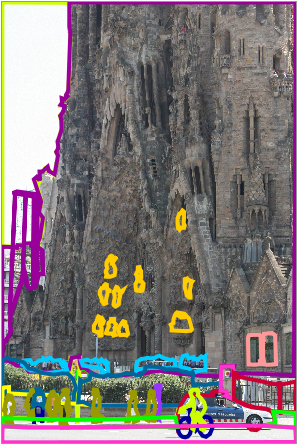
\includegraphics[width=0.80\textwidth]{labelme}
    \caption{LabelMe annotation example \textit{(taken from \url{http://labelme2.csail.mit.edu/})}}
    \label{fig:labelme}
\end{figure}

\begin{figure}[!htb]
  \centering
  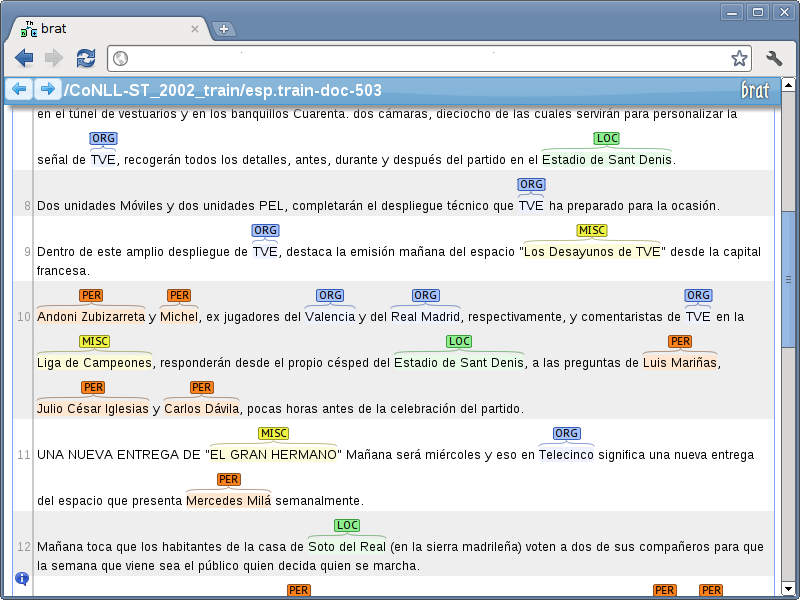
\includegraphics[width=0.80\textwidth]{brat}
    \caption{BRAT \textit{(taken from \url{http://brat.nlplab.org})}}
    \label{fig:brat}
\end{figure}

Similar tools for dataset creation exist in other domains. One example is an image annotation tool called \textbf{LabelMe}\footnote{\url{http://labelme2.csail.mit.edu/}} \cite{labelme} (see figure \ref{fig:labelme}). It is used in object detection and recognition research. Creation of ground-truth data is done through the website. Users upload images and annotate different parts of them by assigning labels like ``tree'', ``window'', ``person'', or some other.

Another is \textbf{brat rapid annotation tool (BRAT)}\footnote{\url{http://brat.nlplab.org}} -- a web-based tool for text annotation, used in natural language processing (NLP) field \cite{brat} (see figure \ref{fig:brat}). It attempts to provide an intuitive and user-friendly with a goal of making annotation more accessible to non-technical users and improving annotation productivity.

\subsection{Evaluation}

Sturm in \cite{sturmfuture} makes several suggestions for improving scientific research in MIR, including some related to evaluation and analysis of results:
\begin{itemize}
    \item Analysis that answers a question of how well the ground-truth of a dataset is shallow and has limited use. This kind of analysis doesn't provide knowledge how the system is operating or whether its performance is satisfactory for a particular use case. The aim should be to produce knowledge, not publication arising from statistical significance.
    \item Acknowledge limitations that all experiments have when drawing any conclusions from them, and to be suspicious of results because some of them seem too good to be true.
    \item Make the work reproducible. It's important to publish and make accessible enough code and resources that were used for evaluation, testing, and other stages of work. Though sometimes, even when this is done, there are errors or other issues that cause the system to produce different results.
\end{itemize}
He also analyzed methods that are used during evaluation (focused on MGR) and showed that ``classification accuracy is not enough'' \cite{sturm2013}.

\section{AcousticBrainz}
\label{sec:soa:acousitcbrainz}

\subsection{Project summary}

As described in section~\ref{sec:motivation}, AcousticBrainz project collects acoustic information which is extracted from users' music collections using the client application \cite{porter2015acousticbrainz}. At the moment of writing it contained more than 2.2 million unique and 4.1 million total submissions from the community.

\subsection{Audio descriptors}

When users run AcousticBrainz client on their audio files, it extracts a set of \textbf{low-level descriptors} using Essentia library \cite{essentia}. Low-level data includes acoustic descriptors which characterize overall loudness, dynamics and spectral shape of a signal, rhythm descriptors, and tonal information.

In addition to low-level descriptors, client submits metadata about a recording:
\begin{itemize}
    \item Codec information and sampling rate
    \item Length of a recording
    \item Version of extractor
    \item Recording name and its \textbf{MusicBrainz Identifier (MBID)}\footnote{\url{https://musicbrainz.org/doc/MusicBrainz_Identifier}}
    \item Artist name and their MBID
    \item ...and other information that is stored in file's tags.
\end{itemize}
Recording MBID might be the most important piece of metadata. All user submissions are recordings that need to be tagged with an MBID. This can be done with one of taggers like MusicBrainz Picard\footnote{\url{https://picard.musicbrainz.org/}}. MBIDs are permanent identifiers that allow to lookup data on MusicBrainz and other projects that support them.

Based on low-level data AcousticBrainz server computes a number of \textbf{high-level descriptors} from low-level data using machine learning models. These are descriptors like timbre, gender, mood, genre, etc.

\section{Conclusions}

\subsection{MIREX}

MIREX is a great framework that encourages advancements in the MIR field by providing a broad set of evaluation tasks\footnote{\url{http://www.music-ir.org/mirex/wiki/2016:Main_Page#MIREX_2016_Possible_Evaluation_Tasks}}. Unfortunately, it's not very flexible to have only one set of challenges per year. This makes it hard to quickly iterate on results, which significantly slows down the research process. Having a framework that can automate or simplify common tasks that are done to prepare such challenge can be very beneficial for the MIR community.

As pointed out in the overview paper \cite{downie2008mirex}, it is difficult to acquire, validate, and store test collections and ground-truth data, which is essential for development of MIR systems. The biggest reason is the current state of copyright in the music industry. There needs to be an easy way to store and share datasets with other researchers.

\subsection{Datasets}

\subsubsection{Creation}

Datasets that are currently used in MIR have a number of problems. These, of course, don't apply to every dataset out there, but most do have some of them.
\begin{itemize}
    \item Size is too small to get good results using machine learning algorithms.
    \item Outdated and don't include new recordings.
    \item Mislabelings, repetitions, bias and other issues with content.
\end{itemize}

As motivation for creation of The Million Song Dataset \cite{millionsongdataset} describes, there are several advantages to creating a large dataset:
\begin{itemize}
    \item It helps reveal problems with scaling of algorithms, which is critical for ``real-world'' use.
    \item Some phenomena or patterns might not be discernible in a small dataset.
    \item It can be more comprehensive, include more specific subsets.
    \item When freely-available, directly promotes comparison of usage results and interchange of ideas.
\end{itemize}

Significant number of datasets are based on crowd-sourced annotations from services like Last.fm\footnote{\url{https://www.last.fm/}} and beaTunes\footnote{\url{https://www.beatunes.com/}} \cite{schreiber2015}. MusicBrainz -- a popular music encyclopedia -- allows editors to assign tags to different entities in the database\footnote{\url{https://musicbrainz.org/doc/MusicBrainz_Entity}}. Most of these services allow users to vote on tags or submit already existing tags. This information can be used to determine which tags are more agreed upon than others, and to automate generation of datasets.

Creation of datasets should be a simple process. As mentioned before, tools for annotation (labeling) exist in other domains. These tools simplify annotation which ultimately improves quality of datasets produced from them. Some lessons can be learned from how they work and be applied to MIR research. While we already have datasets based on annotations from services like Last.fm, it can be useful to streamline this process of generating datasets from different sources.

Simplicity is also important in cases when users have to work with these datasets. This includes tasks like organizing contents and making sure that structure is correct, exporting datasets to perform analysis in some other tools, importing datasets that were created externally into a central repository (AcousticBrainz).

Bias in the process of creation of datasets can be avoided by allowing people to work collaboratively and by integrating user feedback from results of evaluation.
